\chapter{CASE STUDY: HURRICANE HELENE – TESTING THE IMPROVED PARAMETRIZATION}
\label{ch:hurricanes}
This chapter examines the results of the optimal configuration of the cold pool parameterization parameters, the impact of the parameterization itself, and an increase in horizontal resolution during another North Atlantic Basin hurricane season in 2024: Helene. The storm occurred between September 24 and September 27. As in previous analyses, we begin with a description of the event, followed by results categorized into three main features: trajectory, intensity, and rainfall, under the workflow outlined in section \ref{ch:methods}. By the end of the section, we will discuss the findings in detail.

\section{Event description - Helene}

Hurricane Helene was a destructive and rapidly intensifying tropical cyclone that hugely impacted the southeastern United States in late September 2024. Originating in the Central American Gyre (western Caribbean), Helene was first classified as a tropical storm at 0600 UTC on 25 September, approximately 50 nautical miles east of Cozumel, Mexico. Figure \ref{fig:besthelene} show the best track trajectory made by the hurricane.

\begin{figure}[!ht]
	\centering
	\caption{Best track trajectory of Hurricane Helene (September 2024)} % Título acima da figura
	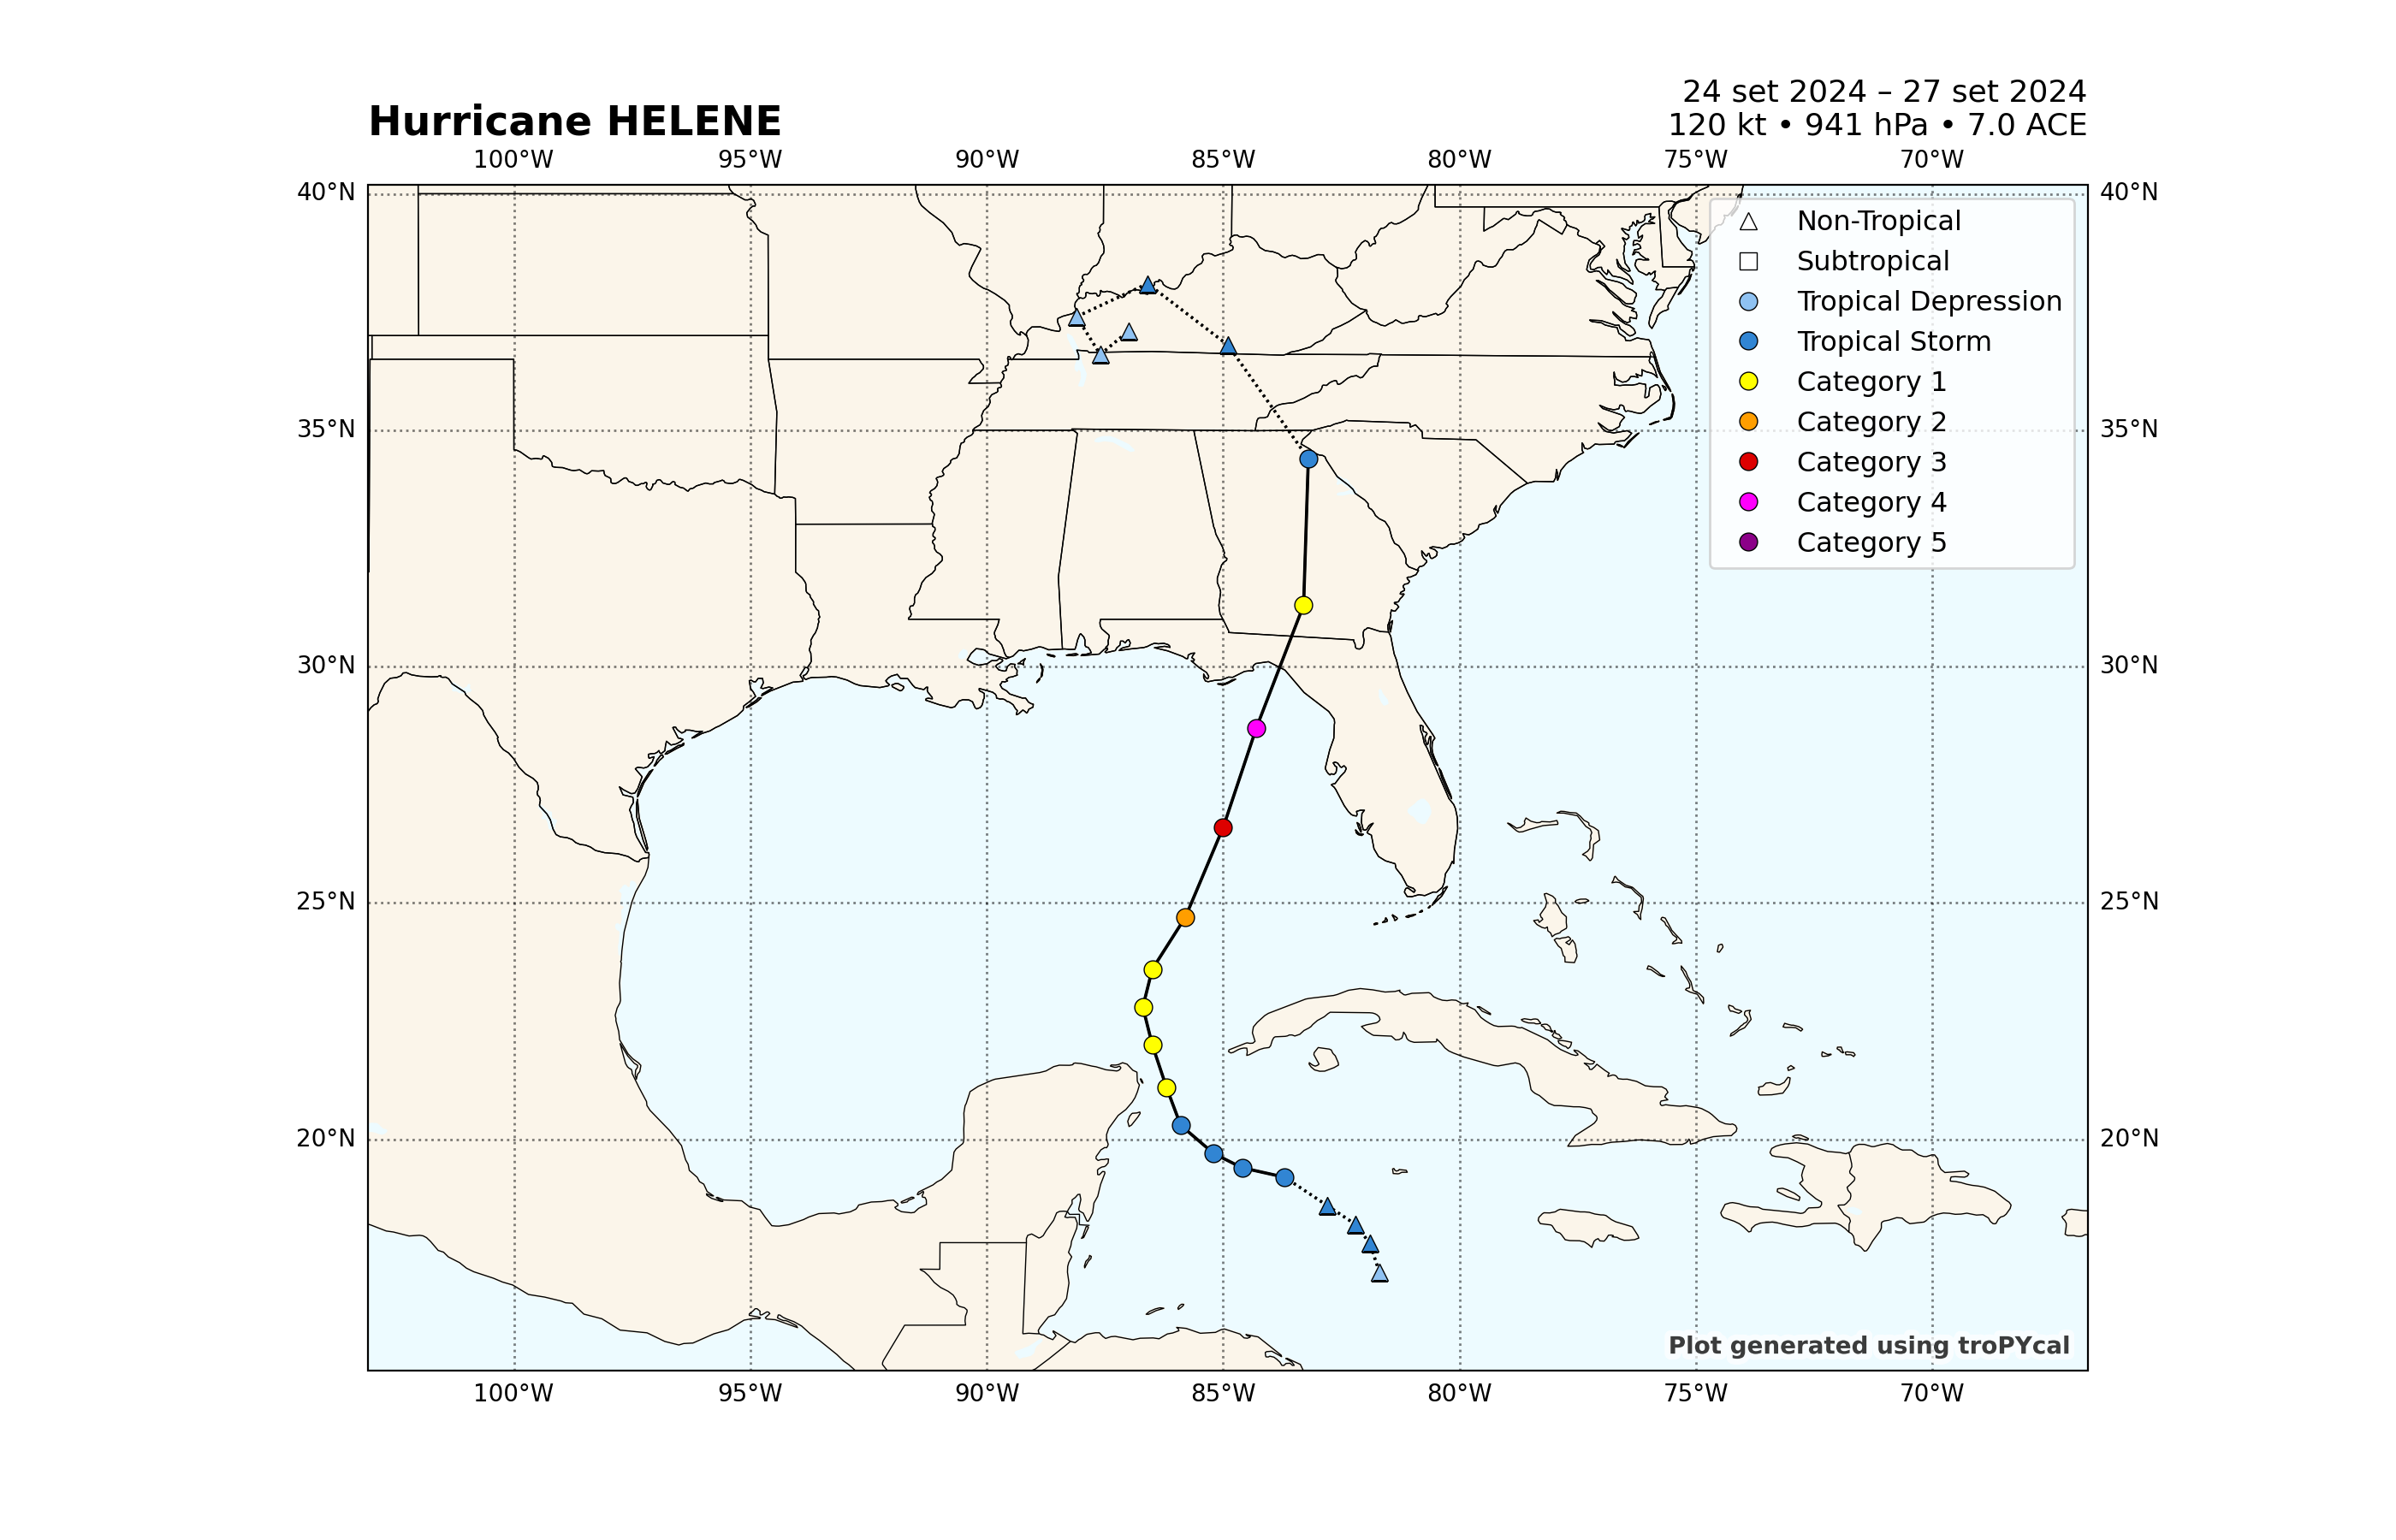
\includegraphics[width=\textwidth, trim= 10 20 10 10, clip]{docs/figuras/chapter6/Helene_2024.png} 
	\vspace{0.5em}
	Source: Made by the author (2025).  % Fonte abaixo da imagem
	\label{fig:besthelene} % Label para referenciar no texto
\end{figure}

By 1200 UTC the same day (25 September), Helene steadily strengthened in conducive environmental conditions of low wind shear, high moisture, and very warm sea surface temperatures, intensifying into a hurricane just east of Cancún by 1800 UTC. It later entered the Gulf of Mexico as a category 1 system on the Saffir-Simpson Hurricane Wind Scale.

Helene’s intensification was notably rapid, surpassing the threshold for rapid intensification (>35 mph increase in wind speed in 24 hours \cite{nhc_helene2024}). Just six hours later, it reached its peak intensity as a category 4 hurricane, with sustained winds of 120 kt (140 mph), approximately 80 nautical miles south-southwest of the Florida Big Bend region.

The first landfall occurred near Perry, Florida, at approximately 0310 UTC on 27 September. At the time, Helene maintained its category 4 status and was moving rapidly north-northeastward. The storm brought catastrophic storm surge to coastal communities, with inundation levels reaching 12 to 16 feet (3.7 - 4.9 meters) above ground level in the Big Bend region, particularly devastating Keaton Beach and Steinhatchee. Additional surge heights of 6 to 8 feet (1.8 - 2.4 meters) were observed as far south as Tampa \cite{fsu_helene2024}.

As Helene moved inland on the morning of 27 September, it gradually weakened due to land interaction. By 0900 UTC, the system had been downgraded to a tropical storm while located near Macon, Georgia. Despite the weakening, Helene’s impacts intensified as the storm interacted with a stationary frontal boundary stretching from the central Gulf Coast to the southern Appalachians. Enhanced low-level convergence and orographic lift contributed to excessive rainfall, particularly in these mountainous regions. Figure \ref{fig:synoptic} pictures this large-scale interation.

\begin{figure}[!ht]
	\centering
	\caption{Synoptic-scale interaction between Hurricane Helene and a stationary frontal boundary over the southeastern U.S} % Título acima da figura
	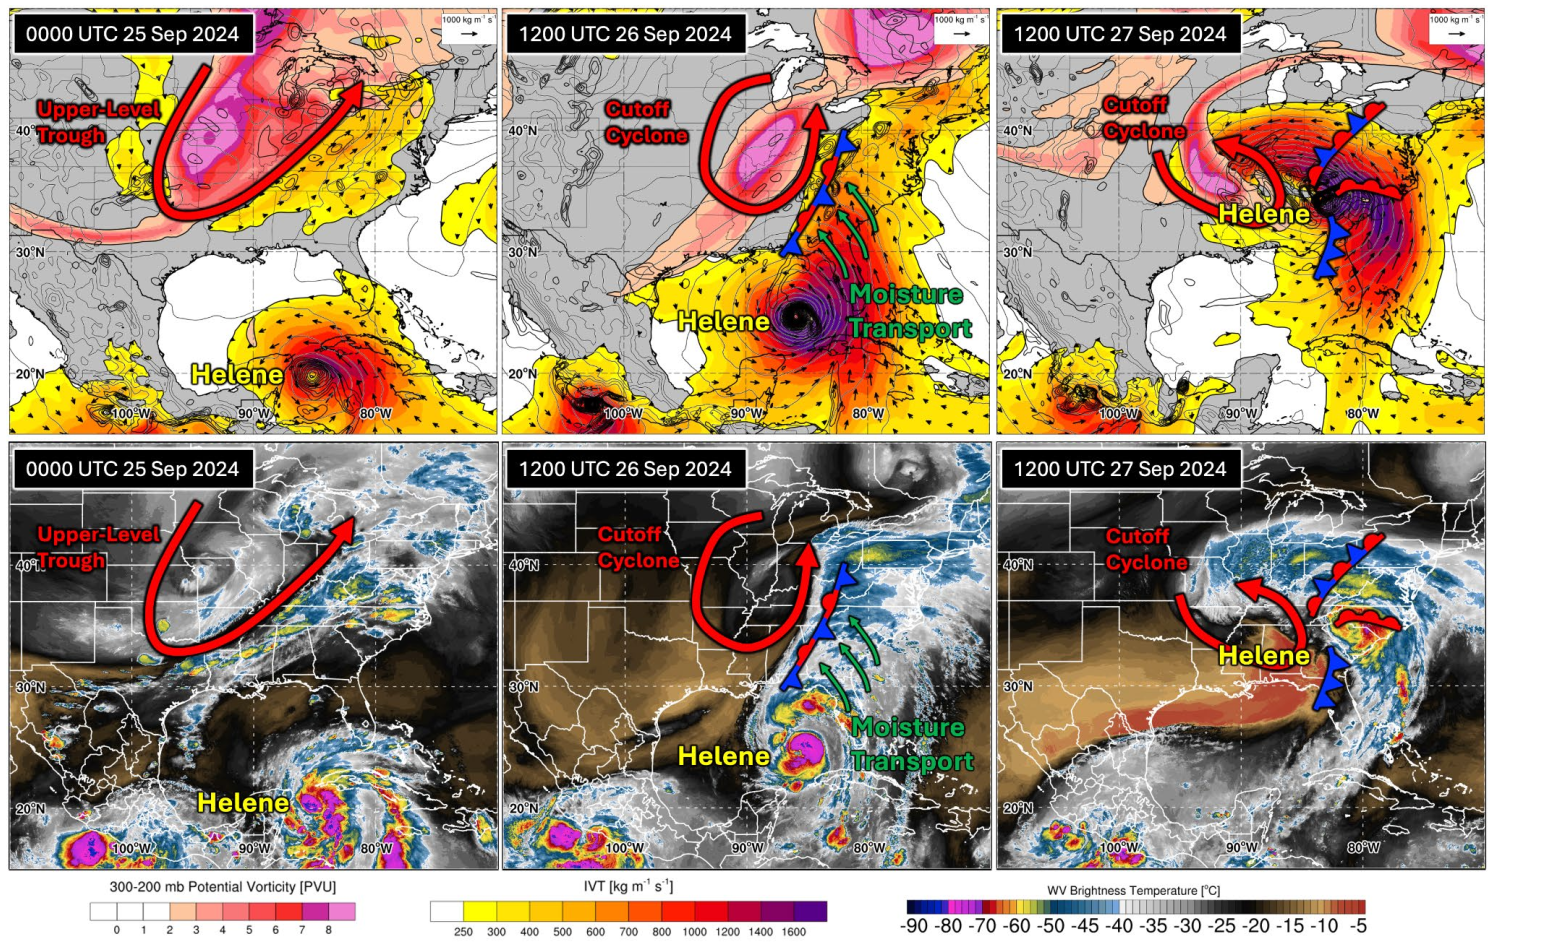
\includegraphics[width=\textwidth]{docs/figuras/chapter6/large_scale_helene.png} 
	\vspace{0.5em}
	Source: \cite{nhc_helene20241}.  % Fonte abaixo da imagem
	\label{fig:synoptic} % Label para referenciar no texto
\end{figure}

Helene’s moisture-laden circulation delivered extreme precipitation across a broad swath of the southeastern United States. The heaviest observed rainfall total was recorded in Busick, North Carolina, where 30.78 inches (approximately 782 mm) fell between 25 and 28 September. The orographic influence was particularly evident in areas such as Georgia and western North Carolina, where intense rainfall led to flash flooding, river overflow, and landslides. A satellite image in Figure XXX shows Helene and the large tail of convection when passing thought North Carolina.

\begin{figure}[h!]
	\centering
	\caption{Satellite images of Hurricane Helene with trailing convection over North Carolina.}
	\begin{minipage}[t]{0.45\textwidth}
		\centering
		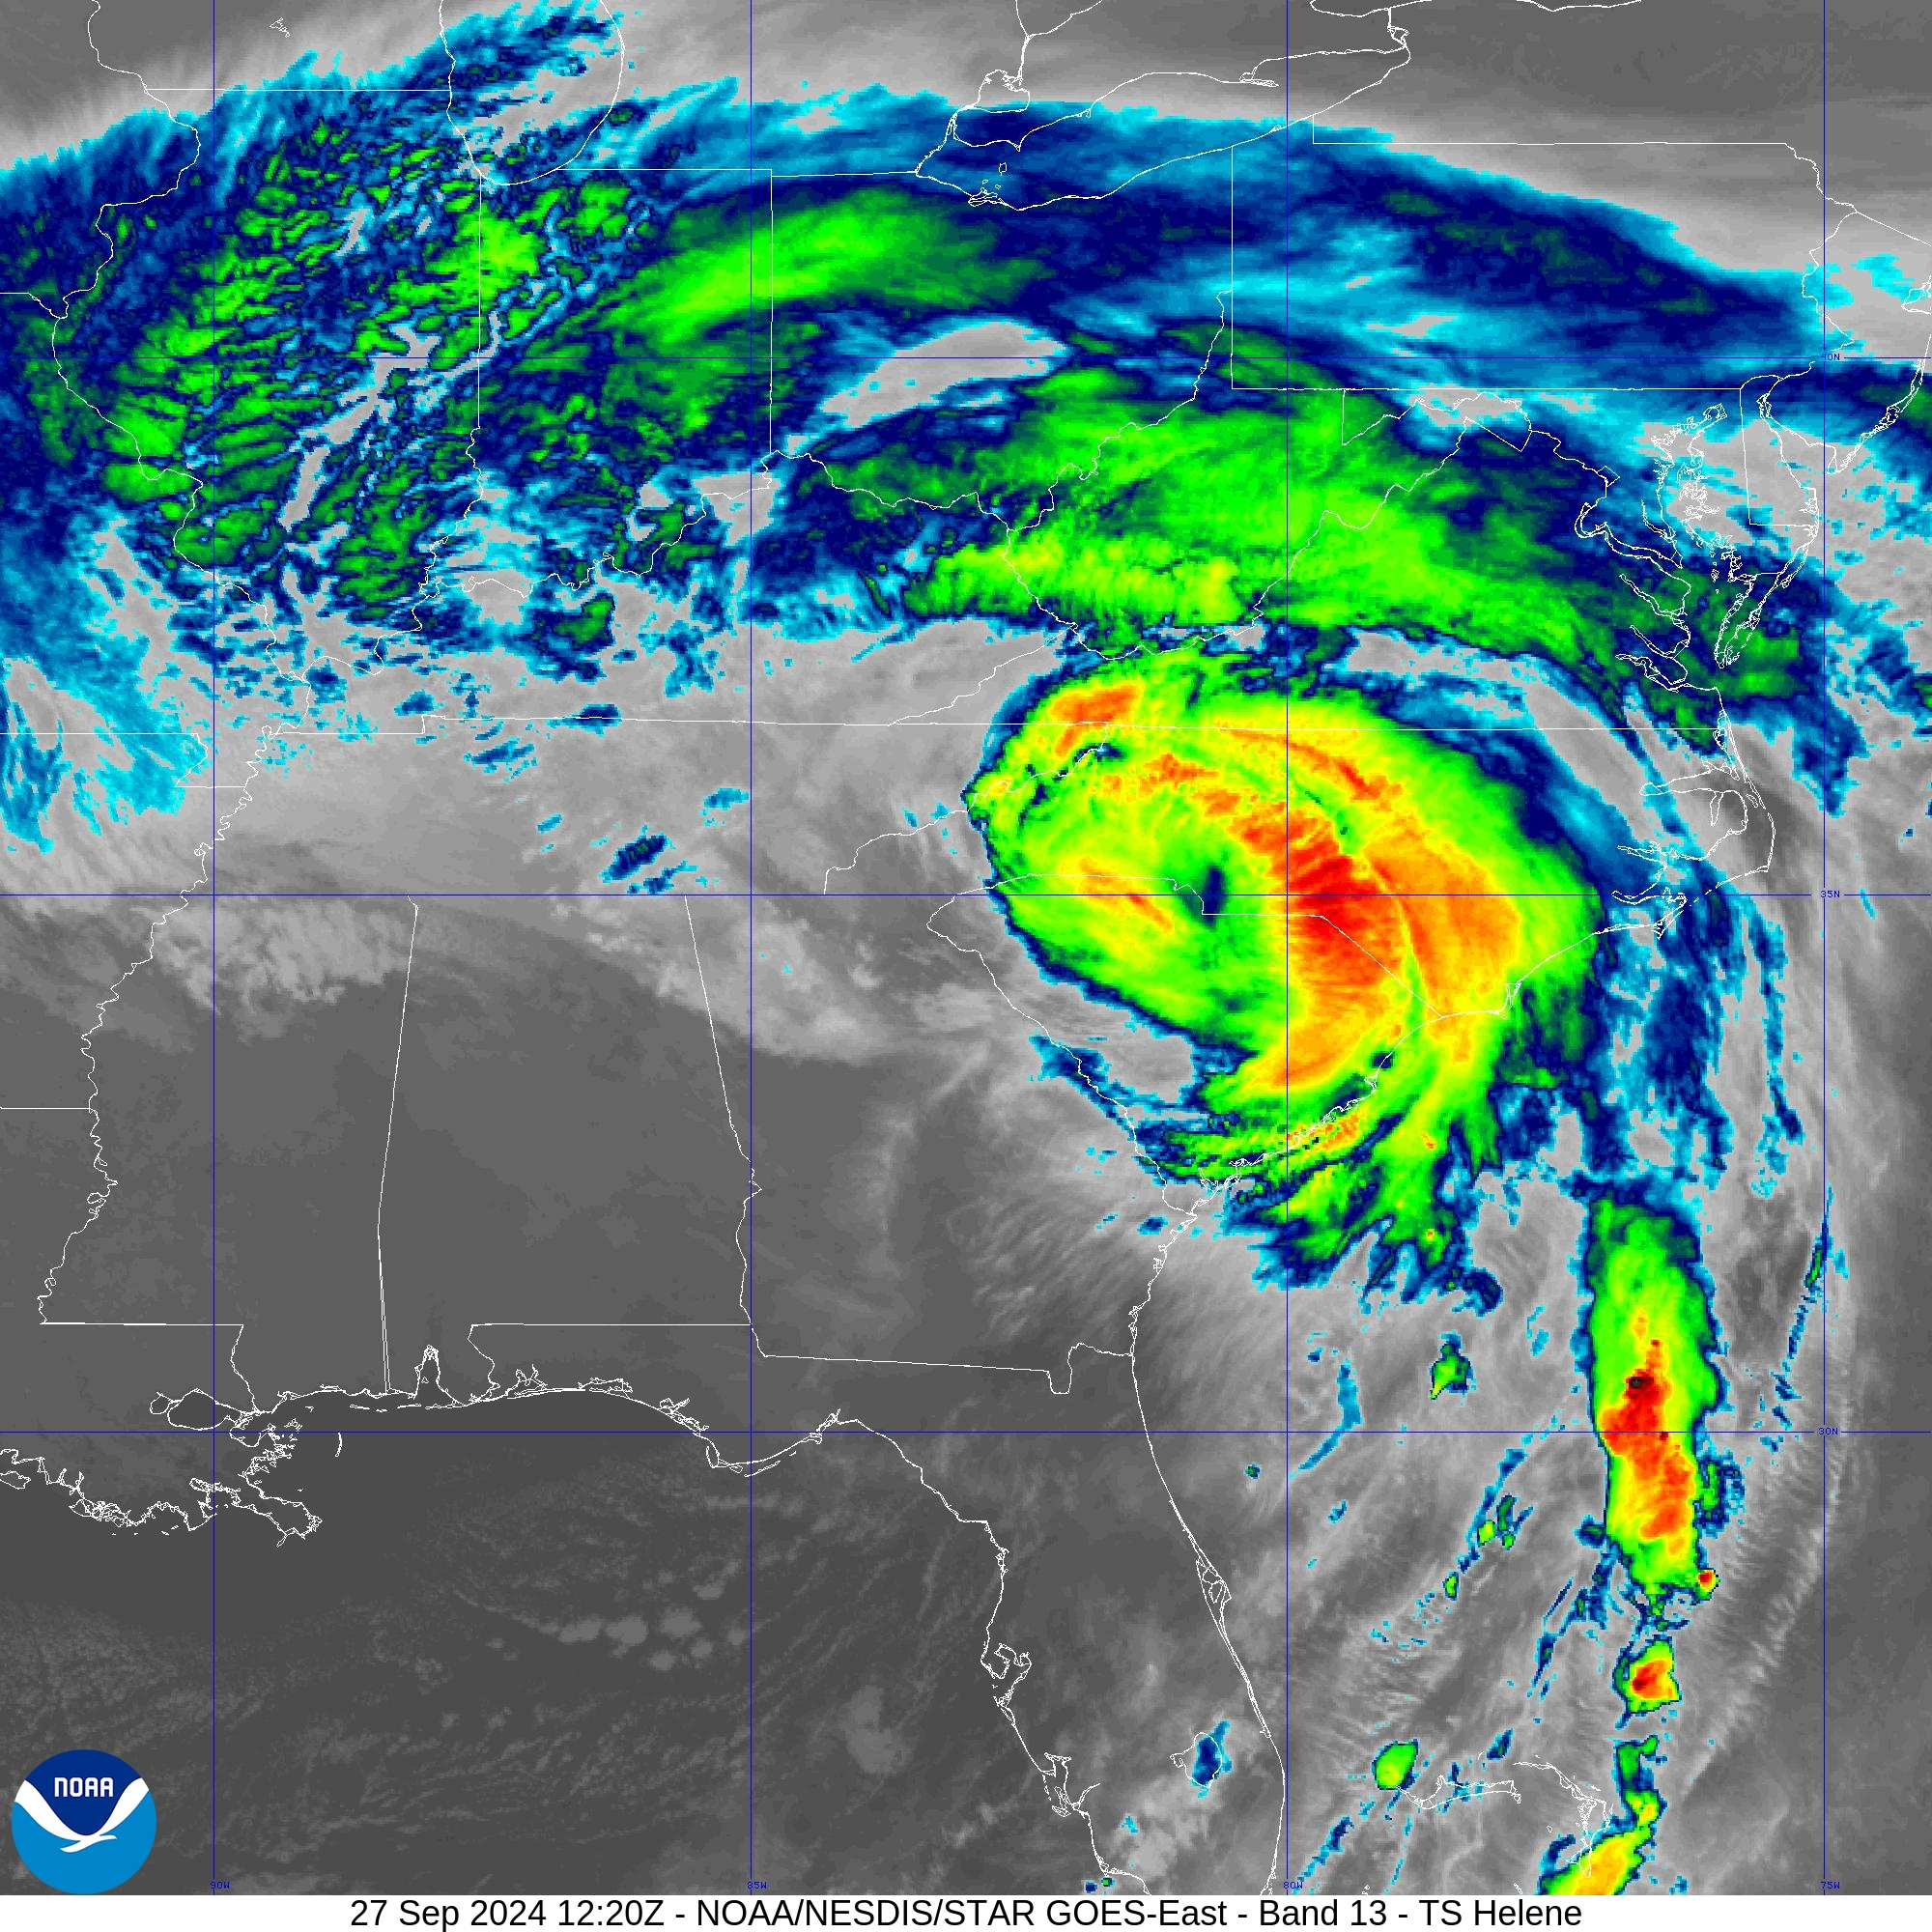
\includegraphics[width=\textwidth]{docs/figuras/chapter6/20242711220_GOES16-ABI-FL-13-AL092024-2000x2000.jpg}
	\end{minipage}\hfill
	\begin{minipage}[t]{0.45\textwidth}
		\centering
		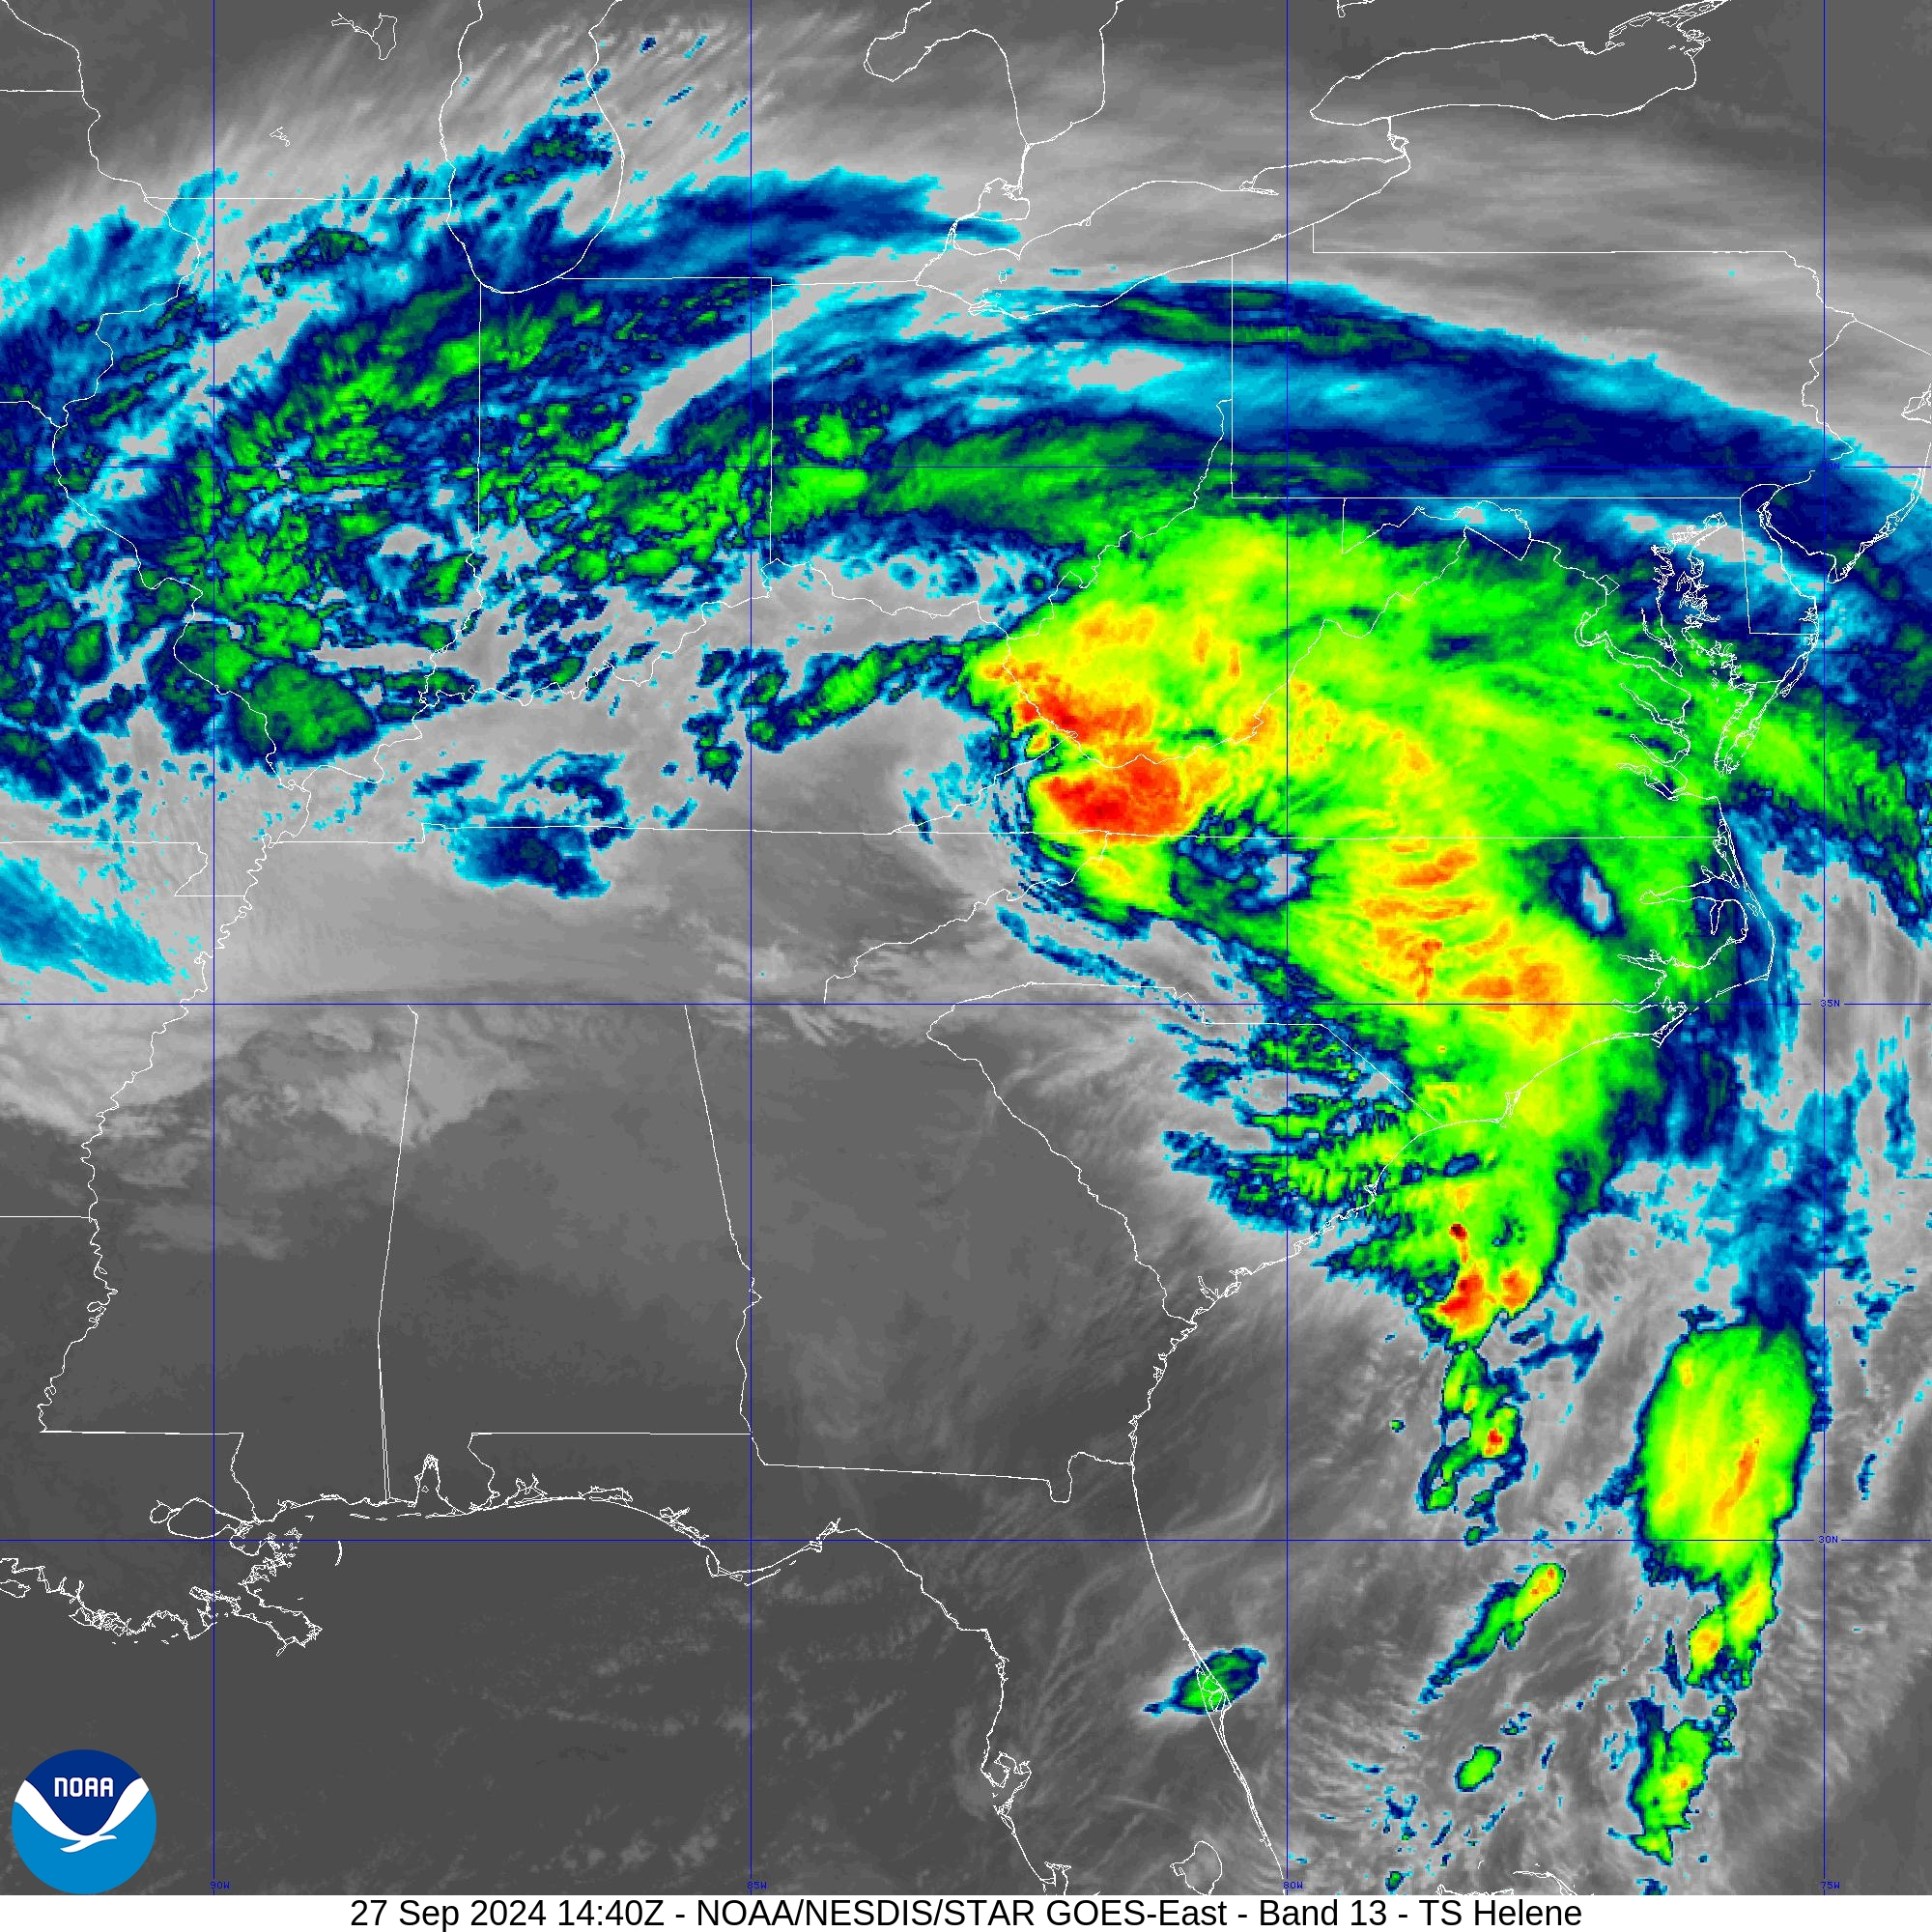
\includegraphics[width=\textwidth]{docs/figuras/chapter6/20242711440_GOES16-ABI-FL-13-AL092024-2000x2000.jpg}
	\end{minipage}
	
	\vspace{0.5em}
	
	\label{fig:northcarolina}
	
	\centering
	Source:.
\end{figure}

The small mountain town of Chimney Rock, NC, was among the hardest hit, with floodwaters destroying much of the local infrastructure \cite{britannica_helene}. Table \ref{tab:highest_rainfall_state} summarizes the total rainfall by state.

\begin{table}[]
	\centering
	\caption{Highest Rainfall Totals by State}
	\label{tab:highest_rainfall_state}
	\resizebox{\textwidth}{!}{
		\begin{tabular}{llll}
			\toprule
			\textbf{State} & \textbf{County} & \textbf{Location} & \textbf{Rainfall (inches)} \\
			\midrule
			North Carolina & Yancey   & Busick                & 30.78 \\
			South Carolina & Greenville & Sunfish Mountain     & 21.66 \\
			Georgia        & Rabun    & 3.5 mi NE Dillard      & 14.64 \\
			Florida        & Liberty  & Sumatra                & 14.39 \\
			Tennessee      & Johnson  & Trade                  & 10.98 \\
			Virginia       & Grayson  & 5.3 mi SW Galax        & 10.89 \\
			Ohio           & Scioto   & Rosemount              & 8.51  \\
			Alabama        & Houston  & 1.6 mi NNE Pansey      & 8.50  \\
			Kentucky       & Henderson & Henderson             & 7.67  \\
			Illinois       & Massac   & Ft. Massac St. Park    & 7.47  \\
			West Virginia  & Mercer   & Bluefield              & 6.11  \\
			Indiana        & Clark    & 2.6 mi E Henryville    & 5.69  \\
			\bottomrule
		\end{tabular}
	}
	
	\vspace{2mm}
	{\centering Source: \cite{nhc_helene20241}.\par}
\end{table}

By 1800 UTC on 27 September, Helene had become post-tropical as it merged with a mid-latitude cutoff low over the Tennessee Valley and transitioned into an extratropical cyclone over southern Kentucky. The remnant low persisted until 28 September, performing a slow cyclonic loop before dissipating over north-central Tennessee.

Hurricane Helene resulted in widespread devastation across Florida, Georgia, the Carolinas, and Tennessee. Approximately 4 million people lost power due to infrastructure damage. With at least 250 reported fatalities, 176 of which were direct, Helene became the deadliest hurricane in the contiguous United States since Hurricane Katrina in 2005.

For our simulations, we compute the entire period from 24 12UTC September to 27. Following figure XXX, the trajectory in the period of our simulations is represented by….

\begin{figure}[!ht]
	\centering
	\caption{Criar um titulo aqui} % Título acima da figura
	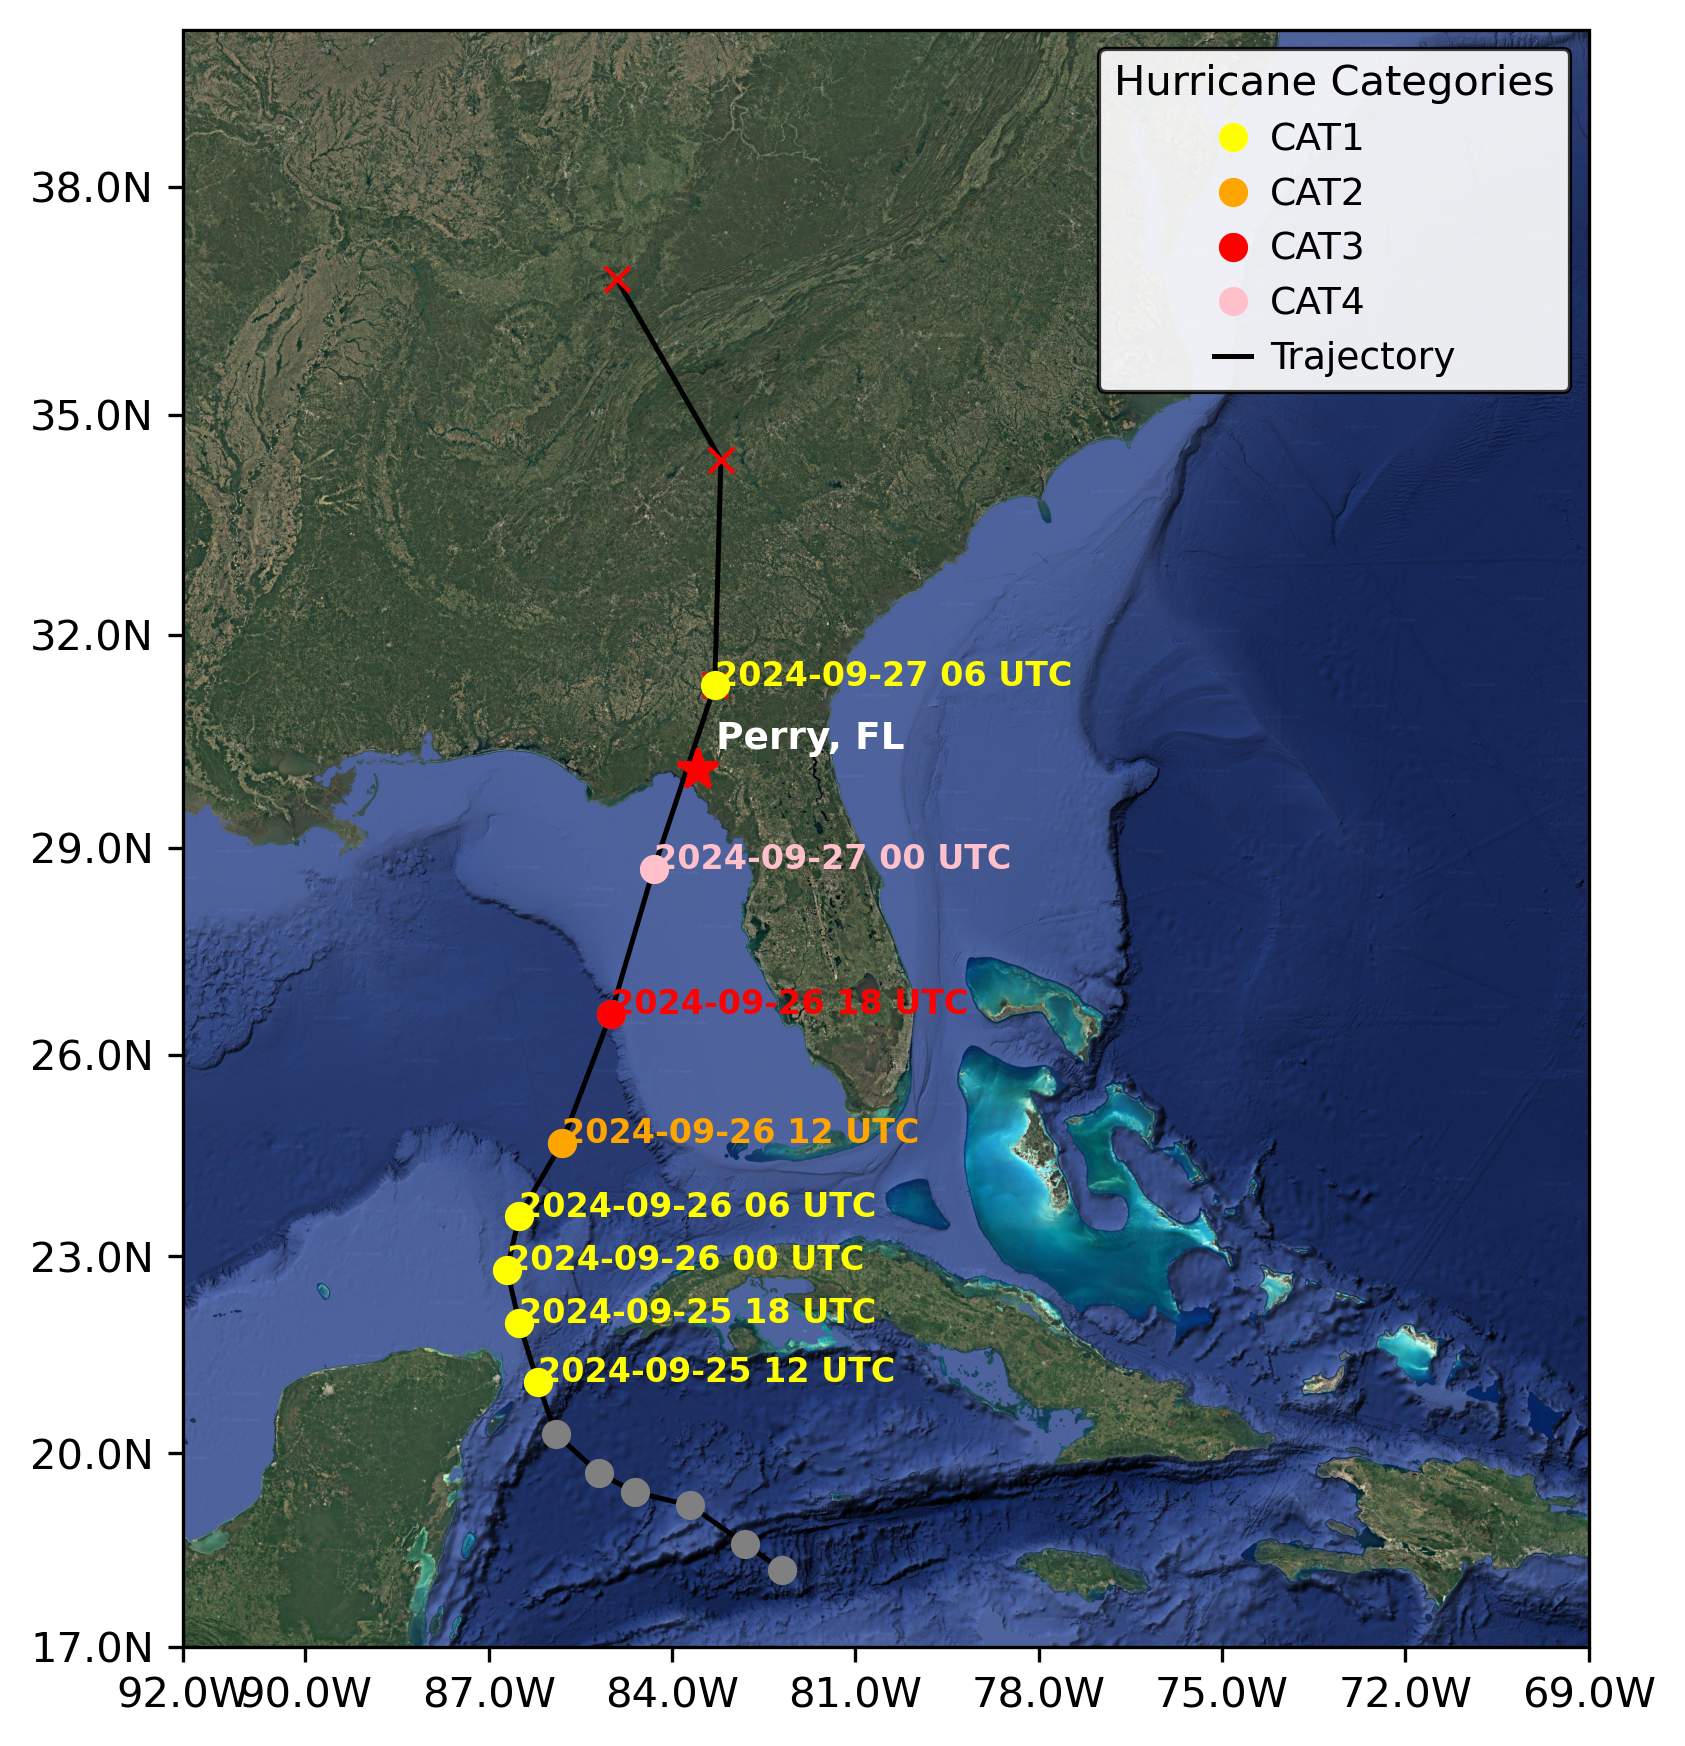
\includegraphics[width=\textwidth]{docs/figuras/chapter6/HELENE_map_with_cat_path.png} 
	\vspace{0.5em}
	Source: .  % Fonte abaixo da imagem
	\label{fig:synoptic} % Label para referenciar no texto
\end{figure}



\section{Results and analysis of hurricane Helene}

\subsection{Trajectory}

\subsection{Intensity}

\subsection{Rainfall}

\subsubsection{Pattern and spatial rainfall distribution}

\subsubsection{Rainfall mean and overall distribution}

\subsubsection{MONAN performance at forecasting rainfall}

\section{Discussion of key outcomes}

